In this section, the layer is described in some detail in terms of its specific subsystems. Describe each of the layers and its subsystems in a separate chapter/major subsection of this document. The content of each subsystem description should be similar. Include in this section any special considerations and/or trade-offs considered for the approach you have chosen.

\subsection{MIDI encoder}
The MIDI encoder gets the signal from the laser receptors, converts it to MIDI data and sends to the Raspberry Pi for the output. This converts the laser receptor signals to MIDI data in order to convert it to sound data.  

\begin{figure}[h!]
	\centering
 	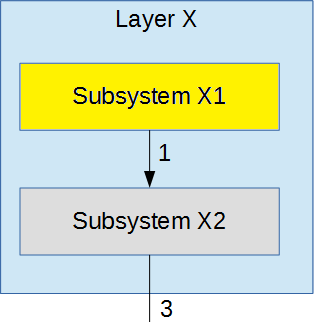
\includegraphics[width=0.60\textwidth]{images/subsystem}
 \caption{MIDI encoder subsystem description diagram}
\end{figure}

\subsubsection{Assumptions}
The MIDI encoder is connected to the Pi and the laser receptors via usb-A cable. It also has a built-in software that converts the data automatically.

\subsubsection{Responsibilities}
The laser recptors, when it detects an interference, sends signal to the MIDI encoder. Here, the encoder converts the signal data it received to a MIDI data so it can be maniplated to different sounds with the sound modules.

\subsubsection{Subsystem Interfaces}
Each of the inputs and outputs for the subsystem are defined here. Create a table with an entry for each labelled interface that connects to this subsystem. For each entry, describe any incoming and outgoing data elements will pass through this interface.

\begin {table}[H]
\caption {Subsystem interfaces} 
\begin{center}
    \begin{tabular}{ | p{1cm} | p{6cm} | p{3cm} | p{3cm} |}
    \hline
    ID & Description & Inputs & Outputs \\ \hline
    \#xx & Description of the interface/bus & \pbox{3cm}{input 1 \\ input 2} & \pbox{3cm}{output 1}  \\ \hline
    \#xx & Description of the interface/bus & \pbox{3cm}{N/A} & \pbox{3cm}{output 1}  \\ \hline
    \end{tabular}
\end{center}
\end{table}


